\newpage
\section{8086 Microprocessor}
The 8086 microprocessor is an enhanced version of the 8085 microprocessor developed by Intel in 1978. It is a 16-bit microprocessor, with 20 address lines and 16 data lines to provide up to 1 MB of physical memory. The 8086 microprocessor described in the project will operate in its minimum mode.

    \begin{figure}[h]
        \begin{center}
            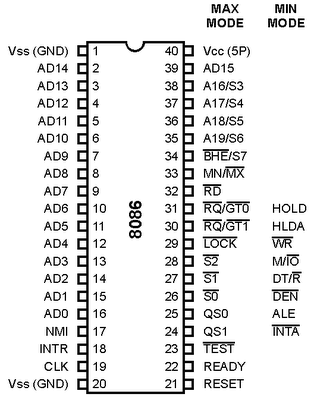
\includegraphics[width=0.35\textwidth]{figures/01_8086.png}
            \caption{8086 Microprocessor} \label{fig:8086}
        \end{center}
    \end{figure}

    \subsection{Features}
    The 8086 microprocessor is known for its significant advancements since its predecessors. The most prominent features include, but are not limited to:

        \begin{itemize}

            \item 6 bytes of cache memory for faster processing

            \item Pipelining stages: Fetch Stage and Execute Stage

            \item Instruction queue

            \item 256 vectored interrupts

            \item Maximum and minimum modes of operation, suitable for multiple and single processors respectively

        \end{itemize}

        \begin{figure}[ht]
            \begin{center}
                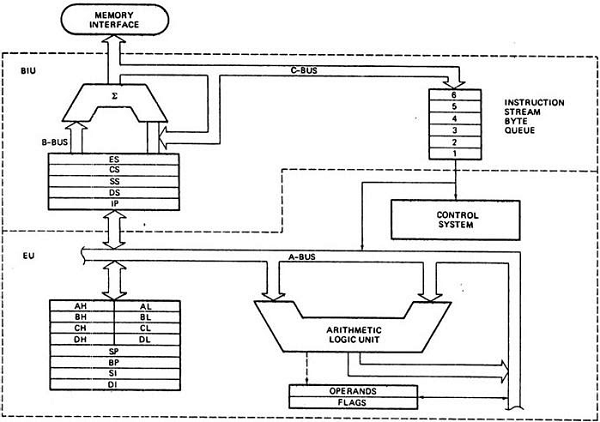
\includegraphics[width=0.65\textwidth]{figures/02_8086_architecture.jpg}
                \caption{Architecture of 8086} \label{fig:8086_architecture}
            \end{center}
        \end{figure}

    \subsection{Address and Data Buses}
    The 8086 CPU has a unidirectional address bus with 20 address lines and a bidirectional data bus with 16 data lines. \cite{buses} The address bus is used to select the desired memory or I/O device by generating a unique address which corresponds to the memory location or the location of I/O device of the system. The data bus is used to transfer data between the CPU and memory and the CPU and I/O devices.\n
    The address bus is denoted as $A_{19}-A_{0}$ (20 lines) and the data bus $D_{15}-D_{0}$ (16 lines). The peripheral devices implemented with the 8086 in this document however consist of 8-bit data bus architectures. The data bus would therefore be multiplexed and more commonly denoted as $D_{7}-D_{0}$ (8 lines).

    \subsection{Control Bus}
    The control bus of 8086 carries control signals which are used to specify the memory and I/O devices. \cite{buses} The bus is bidirectional and assists the CPU in synchronizing control signals to internal devices and external components. It is comprised of interrupt lines, byte enable lines, read/write signals and status lines.
